\documentclass[runningheads,a4paper]{llncs}

\usepackage{amssymb}
\setcounter{tocdepth}{3}
\usepackage{graphicx}
\usepackage{calc,listings,color}

\usepackage{url,xspace}

\newcommand{\linboxsp}{{\sc LinBox}\xspace}
\newcommand{\linbox}{{\sc LinBox}}

\begin{document}

\mainmatter  
\title{\linboxsp memory management and parallel model}
%\titlerunning{}
\author{The \linboxsp group}
\maketitle

\section{Introduction}


\section{A lightweight memory management}

\subsection{Call-by-reference}

Only references as argument (no value returned), first args as return
values.

\verb! Matrix & Function( Matrix & result, const XXX& args); !

example of fields \cite[\S 2.1]{jgd:2002:icms} ?

\subsection{The mother model}


The mother model: functions should not allocate their return values

\begin{itemize}
\item more efficient: allocations are limited

\item requires more involvment by the programmer: control of the allocation

\item garbage collection is simplified: reference counting with a single
boolean, or even better (sic) by two different classes.
Especially for thread-safety.
\end{itemize}


\subsection{Rebind of matrices}

mecanism of the rebind for fields adapted from STL rebind of
allocators.

Since rebind must not allocate, only references are given (re)
allocation is done by the caller (and not rebind), rebind only maps
values from one field to another.

\begin{itemize}
\item generic homomorphism 
\verb!e.init( newelt, e.convert( Integer, oldelt) )!
can be specialized.
\end{itemize}

\section{Abstraction of a level for parallelism}
\subsection{Parallel building blocks}

namespace selection of algorithms like \verb!for_each!,
\verb!transform!, etc. 

\begin{itemize}
\item Transparent parallelism
\item Abstraction of parallelism
\item Parallelism really as a plug-in
\end{itemize}

\subsection{Accumulate-while and early termination}
Proposition of a new algorithm:
\verb!Accumulate-while!, generalization of \cite{jgd:2010:crt},
specially adapted to early termination in mathematical softwares.

Other applications (e.g. from \cite{Beaumont:2004:PMAA}) ??


\subsection{Memory contention}
solved (?) with multi-threaded memory allocators ...

\section{Separate compilation}
One solution for management of code bloat was given via
\verb!Archetypes! in \cite[\S 2.1]{jgd:2002:icms}

Here we propose to automatize \cite{Erlingsson:1996:issac} technique:

\begin{itemize}
\item For a given generic algorithm, e.g. \verb!rank!, we define the
  generic algorithm, and its specializations, to be a generic function
  prefixed with \verb!generic!, not supposed to be directly called. See e.g. 
\verb!template<class Matrix> size_t& generic_rank(size_t& rank, const Matrix& A);!
\item Next we automatically define the user interface in a caller that
  high level users should use:
\begin{verbatim}
template<class Matrix> size_t& rank(size_t& rank, const Matrix& A) {
   return generic_rank(r, A);
}
\end{verbatim}
\item Then the separate compilation specialization can be defined,
  according to a compile time decision, i.e. a macro 
\verb!#define __LINBOX_SEPARATE_COMPILATION!
\begin{itemize}
\item If this macro is not set, leave as it is, it works.
\item Otherwise, define in the library, \verb!liblinbox.a!, 
a specific caller, which will instantiate the generic caller e.g,
\begin{verbatim}
size_t& rankOfDenseMatrixOverGF2(size_t& rank, const DenseMatrix<GF2>& A) {
   return rank_implementation(r, A);
}
\end{verbatim}
and then define a specialization of the user level call:
\begin{verbatim}
template<> size_t& rank(size_t& rank, const DenseMatrix<GF2>& A) {
   return rankOfDenseMatrixOverGF2(r, A);
}
\end{verbatim}
\end{itemize}
\end{itemize}

\begin{itemize}
\item thanks to inlining by compiler, the cost is a single extra
  function call (to the pre-compiled code) and not two.
\item speeds-up external usage such as Maple, Sage interfaces:
  compilation timings ?
\end{itemize}

\begin{figure}[ht]
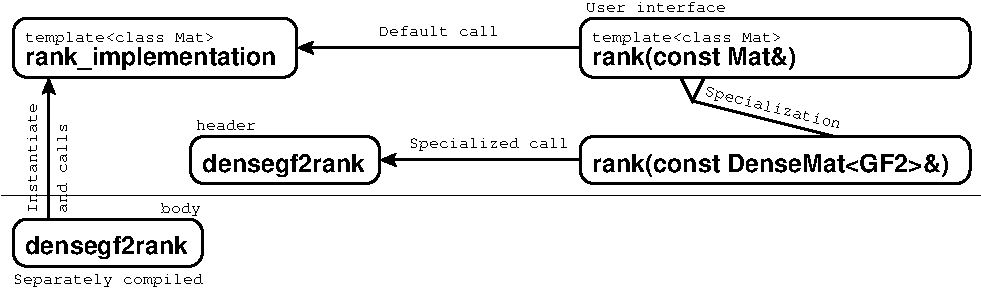
\includegraphics[width=\textwidth]{separate}
\caption{Separate compilation of a rank specialization}\label{fig:sep}
\end{figure}


\bibliographystyle{plain}
\bibliography{jgdbibl} 

\end{document}